\RequirePackage{fix-cm}
\documentclass[12pt]{article}
\renewcommand{\familydefault}{\sfdefault}
%\usepackage[T1]{fontenc}
\usepackage[top=4cm, bottom=4cm, left=4cm, right=4cm]{geometry}
\geometry{a2paper}
\usepackage[parfill]{parskip} % begin paragraphs with an empty line rather than an indent
\usepackage{graphicx}	
\usepackage{amssymb}
\usepackage{tikz}
\usepackage[export]{adjustbox}
\usepackage{eso-pic}
	\newcommand\BackgroundPic{%
	\put(0,0){%
	\parbox[b][\paperheight]{\paperwidth}{%
	\vfill
	\centering
	
\includegraphics[width=\paperwidth,height=\paperheight,keepaspectratio]{background_blank_A4.pdf}%
	\vfill
	}}}
\definecolor{langblue1}{HTML}{00205B} %Pantone 281
\definecolor{langred1}{HTML}{D73367}
\definecolor{langgray1}{gray}{0.65}
\definecolor{langgray2}{HTML}{C7C9C7} %Pantone 420

\begin{document}

\AddToShipoutPicture{\BackgroundPic}
\begin{titlepage}\centering
		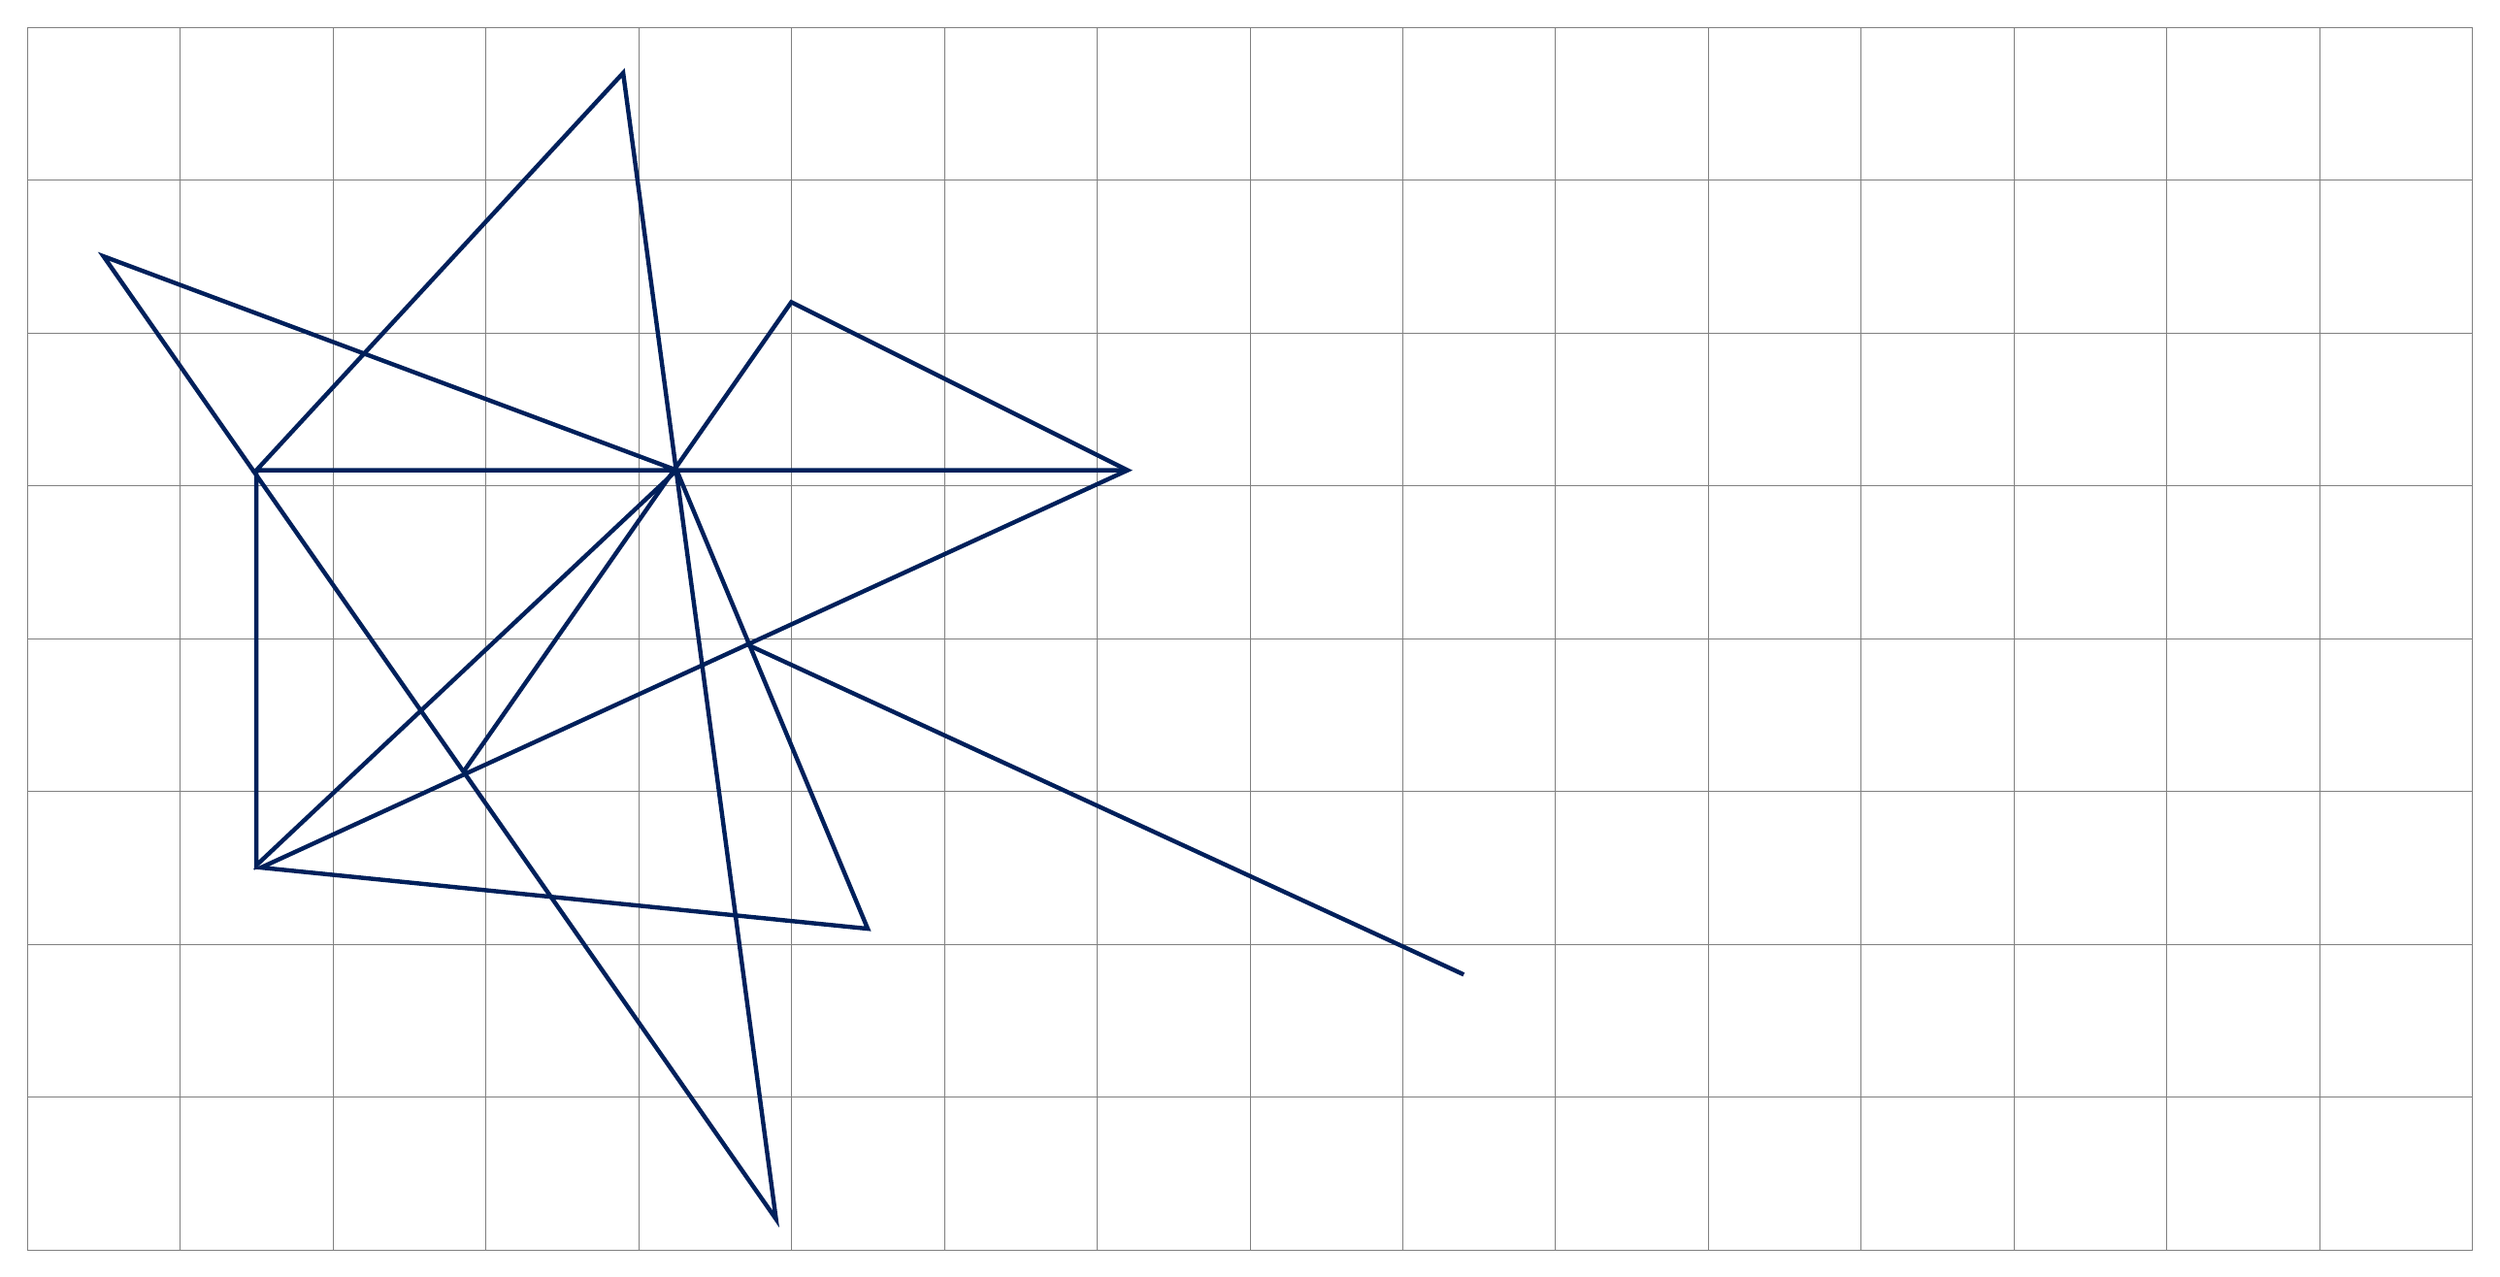
\begin{tikzpicture}[scale=2]
			\draw[help lines] (0,0) grid (16,8);
			\draw[langblue1,ultra thick] (7.2,5.1) -- (1.5,5.1) -- (3.9,7.7) -- (4.9,0.2) -- (0.5,6.5) -- (4.25,5.1) -- (1.5,2.515) -- (1.5,5.1);
			\draw[langblue1,ultra thick] (4.25,5.1) -- (5.5,2.1) -- (1.53,2.5) -- (7.2,5.1) -- (5,6.2) -- (2.85,3.12);
			\draw[langblue1,ultra thick] (4.7,3.965) -- (9.4,1.8);
		\end{tikzpicture}
		
	Workshop \& Conference
	
	March 27-29 2017 \& March 29-31 2017
	
	J-Building, Universit\"{a}t Paderborn
	
	The conference is a platform for researchers from the field of corpus linguistics to discuss current topics and present their projects and latest results. The languages of the conference are English and German.
	
	%{\fontsize{5cm}{5.5cm}\selectfont This is big!}
	
	Confirmed Speakers
	
	Dr.~Sabine Bartsch (TU Darmstadt)
	
	Prof.~Dr.~Klaus P.~Schneider (Universit\"{a}t  Bonn)
	
	Prof.~em.~Dr.~Dr.~h.c.mult.~Norbert Richard Wolf (Emeritus Professor, Universit\"{a}t W\"{u}rzburg)
	
	Organiser
	
	Pro.~Dr.~Ilka Mindt (Universit\"{a}t Paderborn)
	
	For more information, please visit our website:
	
	http://kw.uni-paderborn.de/en/anglistik-amerikanistik/korpora2017/workshop/
		\begin{figure}[b!]
			
\includegraphics[width=0.35\textwidth,right]{UPB_LOGO_GB_CMYK_15.pdf}
		\end{figure}
\end{titlepage}

\end{document}  